\documentclass[11pt,letterpaper]{article}
\usepackage[margin=0.85in,headheight=14pt]{geometry}
\usepackage{amsmath,amssymb}
\usepackage{enumitem}
\usepackage{fancyhdr}
\usepackage{lmodern}
\usepackage[T1]{fontenc}
\usepackage[dvipsnames]{xcolor}
\usepackage[most]{tcolorbox}
\usepackage{pgfplots}
\usepgfplotslibrary{groupplots}
\usetikzlibrary{arrows.meta,positioning,shapes.geometric,calc}
\pgfplotsset{
  compat=1.18,
  every axis/.append style={grid=major, grid style={gray!25}, tick label style={font=\footnotesize},
    label style={font=\small}, title style={font=\small}, legend style={font=\scriptsize}},
}
\definecolor{cA}{HTML}{1F77B4}
\definecolor{cB}{HTML}{FF7F0E}
\definecolor{cC}{HTML}{2CA02C}
\definecolor{cD}{HTML}{D62728}
\definecolor{cE}{HTML}{9467BD}

\pagestyle{fancy}
\fancyhf{}
\lhead{SYDE 556/750 \qquad Practice Test 4}
\rhead{Solutions \& marking guide}
\cfoot{\thepage}
\renewcommand{\headrulewidth}{0pt}

\setlength{\parindent}{0pt}
\setlength{\parskip}{4pt}

\newcommand{\tin}{\tau_{\mathrm{in}}}
\newcommand{\T}{\mathsf{T}}
\newcommand{\ans}[1]{\par\vspace{4pt}{\bfseries #1}\quad}

\newtcolorbox{marking}{colback=blue!3,colframe=blue!40!black,boxrule=0.4pt,left=4pt,right=4pt,top=2pt,bottom=2pt,arc=1pt,fonttitle=\bfseries\small,title=Marking}
\newtcolorbox{trap}{colback=red!4,colframe=red!50!black,boxrule=0.4pt,left=4pt,right=4pt,top=2pt,bottom=2pt,arc=1pt,fonttitle=\bfseries\small,title=Where marks are usually lost}

\begin{document}

\begin{center}
{\Large\bfseries Practice Test 4: Decisions, the LMU, Learning \& Representation --- Solutions}\\[2pt]
Total: 20 marks plus 2 bonus. Curves that come from a simulation use \texttt{pn4\_data/make\_data\_test4.py} (Nengo~4.1).
\end{center}

%=====================================================================
\section*{Question 1 \hfill (4)}

\ans{(a) [2]}
The recurrent transform is $A' = 1$, so $A = (A' - 1)/\tau = \mathbf{0}$: an integrator. The input transform is $B' = 1$, so $B = B'/\tau = 1/0.2 = \mathbf{5\ s^{-1}}$. The system is $\dot x = 5u$.

For $u = 0.1$ the ramp has slope $0.5\ \mathrm{s^{-1}}$.
\begin{itemize}[leftmargin=1.2em]
\item Ignoring the mismatch: $0.5t = 0.9$ gives $t = \mathbf{1.8}$ \textbf{s}.
\item With the offset: the fast input synapse adds $(1 - 0.02/0.2)(0.1) = 0.9 \times 0.1 = 0.09$ within about $3\tin = 60$ ms. So $0.5t + 0.09 = 0.9$ gives $t = 0.81/0.5 = \mathbf{1.62}$ \textbf{s}. Nengo gives $1.55$ s.
\end{itemize}
\begin{marking}
0.5: $A = 0$. \ 0.5: $B = 5$ (not $1$). \ 0.5: $1.8$ s. \ 0.5: $1.62$ s with the offset $0.09$.
\end{marking}

\ans{(b) [2]}
$u = -0.05$: slope $-0.25\ \mathrm{s^{-1}}$ and offset $-0.045$, so $x = -0.9$ at $(0.9 - 0.045)/0.25 = 3.42$ s ($3.6$ s ignoring the offset; Nengo $3.32$ s). Each accumulator ramps and then flattens just beyond $\pm1$, because the neurons saturate at the radius. The decision output stays near $0$ and swings to about $\pm1$ as the accumulator passes $\pm0.9$: at about $1.6$ s for $u = 0.1$ and $3.4$ s for $u = -0.05$. Halving the evidence (and flipping its sign) roughly doubles the decision time.
\begin{center}
\begin{tikzpicture}
\begin{axis}[width=0.9\textwidth, height=6cm, xmin=0, xmax=4, ymin=-1.25, ymax=1.25,
  xlabel={$t$ (s)}, ylabel={decoded value}, legend style={at={(0.5,1.03)}, anchor=south, legend columns=4}, legend cell align=left]
  \addplot[cA, thin] table[x=t, y=acc1] {pn4_data/t4_q1.dat};
  \addplot[cA, very thick] table[x=t, y=out1] {pn4_data/t4_q1.dat};
  \addplot[cD, thin] table[x=t, y=acc2] {pn4_data/t4_q1.dat};
  \addplot[cD, very thick] table[x=t, y=out2] {pn4_data/t4_q1.dat};
  \legend{{accumulator, $u = 0.1$}, {decision, $u = 0.1$}, {accumulator, $u = -0.05$}, {decision, $u = -0.05$}}
  \addplot[gray, dotted, thick, domain=0:4, samples=2, forget plot] {0.9};
  \addplot[gray, dotted, thick, domain=0:4, samples=2, forget plot] {-0.9};
  \draw[gray, dashed] (axis cs:1.62,-1.25) -- (axis cs:1.62,1.25);
  \draw[gray, dashed] (axis cs:3.42,-1.25) -- (axis cs:3.42,1.25);
  \node[font=\scriptsize, anchor=south west, fill=white, inner sep=1pt] at (axis cs:1.64,-1.2) {$1.62$ s};
  \node[font=\scriptsize, anchor=south east, fill=white, inner sep=1pt] at (axis cs:3.4,-1.2) {$3.42$ s};
\end{axis}
\end{tikzpicture}
\end{center}
Ways the decoded output differs from the requested step (any two):
\begin{itemize}[leftmargin=1.2em, itemsep=1pt]
\item It cannot jump. A weighted sum of smooth tuning curves ramps across the threshold over a range of $x$, so the decision ``switches on'' gradually, starting a little before $x = 0.9$.
\item It is not exactly $0$ before the decision. The least-squares fit leaves small wiggles over $|x| < 0.9$, plus spike noise.
\item It does not settle at exactly $\pm1$: it undershoots the corner ($-0.85$ here) or overshoots slightly ($1.01$).
\item It lags the accumulator by the connection's synapse.
\end{itemize}
\begin{marking}
0.5: both accumulators ramp, with the steeper one for $u = 0.1$, and flatten at about $\pm1$. \ 0.5: the decision times are about $1.6$ s and $3.4$ s, with the decision at $0$ beforehand. \ 1: two valid differences, $0.5$ each.
\end{marking}
\begin{trap}
Using $B = 1$, which predicts $9$ s for the decision. With \texttt{transform=1} the input gain is $B'/\tau$. Also, drawing the decision output as a clean step from $0$ to $1$.
\end{trap}

%=====================================================================
\section*{Question 2 \hfill (4)}

\ans{(a) [2]}
$\tau A = (\tau/\theta)(\theta A) = 0.2\,(\theta A)$, so
\[
A' = 0.2\,(\theta A) + I = \begin{pmatrix} 0.8 & -0.2 & -0.2 \\ 0.6 & 0.4 & -0.6 \\ -1 & 1 & 0 \end{pmatrix}\ (3 \times 3), \qquad
B' = 0.2\,(\theta B) = \begin{pmatrix} 0.2 \\ -0.6 \\ 1 \end{pmatrix}\ (3 \times 1).
\]
\begin{marking}
1: $A'$ with the $+I$ on the diagonal (deduct $0.5$ for one wrong entry). \ 1: $B'$ with shape $3 \times 1$.
\end{marking}
\begin{trap}
Forgetting the $1/\theta$: $A = (\theta A)/\theta = 4\,(\theta A)$. Using $\tau(\theta A)$ instead gives $0.05$ instead of $0.2$ for the scale.
\end{trap}

\ans{(b) [2]}
\[
u(t - r\theta) \approx 0.5 + 0.3(2r - 1) - 0.2(6r^2 - 6r + 1) = \mathbf{1.8r - 1.2r^2}.
\]
\begin{itemize}[leftmargin=1.2em, itemsep=1pt]
\item Now ($r = 0$, using $\tilde P_i(0) = (-1)^i$): $0.5 - 0.3 - 0.2 = \mathbf{0}$.
\item $\theta$ ago ($r = 1$, using $\tilde P_i(1) = 1$): $0.5 + 0.3 - 0.2 = \mathbf{0.6}$.
\item Average: only $\tilde P_0$ has a nonzero integral, so the average is $x_0 = \mathbf{0.5}$. Check: $\int_0^1(1.8r - 1.2r^2)\,dr = 0.9 - 0.4 = 0.5$.
\end{itemize}
The stored window is a parabola: $0$ now, peaking at $0.675$ at $r = 0.75$ ($\theta' \approx 0.19$ s), and $0.6$ at $0.25$ s ago. The input was larger in the recent past and has fallen to $0$.
\begin{center}
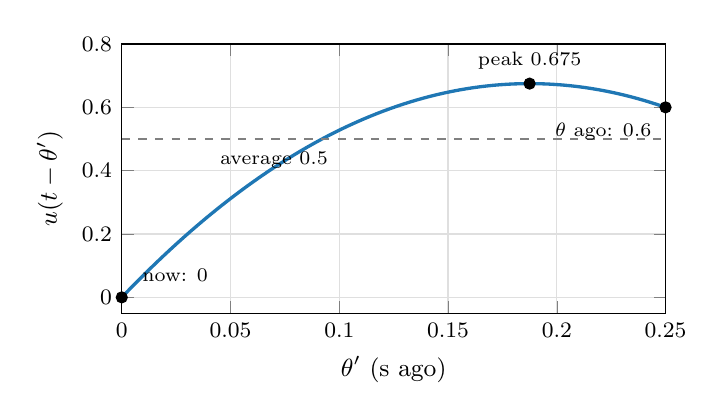
\begin{tikzpicture}
\begin{axis}[width=0.7\textwidth, height=5cm, xmin=0, xmax=0.25, ymin=-0.05, ymax=0.8,
  xlabel={$\theta'$ (s ago)}, ylabel={$u(t - \theta')$}, scaled x ticks=false,
  xticklabel style={/pgf/number format/fixed}]
  \addplot[cA, very thick, domain=0:0.25, samples=80] {1.8*(x/0.25) - 1.2*(x/0.25)^2};
  \addplot[gray, dashed, domain=0:0.25, samples=2] {0.5};
  \addplot[only marks, mark=*, black] coordinates {(0,0) (0.25,0.6) (0.1875,0.675)};
  \node[font=\scriptsize, anchor=south west] at (axis cs:0.005,0.02) {now: $0$};
  \node[font=\scriptsize, anchor=north east] at (axis cs:0.248,0.58) {$\theta$ ago: $0.6$};
  \node[font=\scriptsize, anchor=south] at (axis cs:0.1875,0.69) {peak $0.675$};
  \node[font=\scriptsize, anchor=north] at (axis cs:0.07,0.49) {average $0.5$};
\end{axis}
\end{tikzpicture}
\end{center}
\begin{marking}
0.5: $1.8r - 1.2r^2$. \ 0.5: now $= 0$. \ 0.5: $\theta$ ago $= 0.6$ and average $= 0.5$. \ 0.5: sketch starts at $0$, rises to a hump near $0.19$ s, and ends at $0.6$.
\end{marking}

%=====================================================================
\section*{Question 3 \hfill (4)}

\ans{(a) [2]}
\[
\langle e_1, \varepsilon\rangle = 0.06 - 0.16 = -0.1, \qquad \Delta w_{1j} = -10^{-4}(2)(-0.1)(50) = \mathbf{+0.001},
\]
\[
\langle e_2, \varepsilon\rangle = 0.08 + 0.12 = +0.2, \qquad \Delta w_{2j} = -10^{-4}(2)(0.2)(50) = \mathbf{-0.002}.
\]
The error is actual $-$ target. Along $e_2$ the output is too large, so neuron 2, which pushes the output along $e_2$, receives less drive. Along $e_1$ the output is too small, so neuron 1 receives more. Both changes move the decoded output against the error.
\begin{marking}
0.5 each: both projections. \ 0.5: both $\Delta w$ values with the correct signs. \ 0.5: the explanation in terms of each encoder's projection of the error.
\end{marking}

\ans{(b) [2]}
\begin{itemize}[leftmargin=1.2em, itemsep=1pt]
\item \textbf{Just after $t = 0$:} the output is $0$, so the error is the whole target and the RMSE $\approx$ the input RMS, $\mathbf{0.5}$. (A short window can read a little lower; Nengo's first $0.5$ s gives $0.36$.) It then decays roughly exponentially over a few seconds to a floor of about $0.05$, never zero (finite neurons and spike noise).
\item \textbf{Just after $t = 10$ s:} the output is about $x$ and the target is $-x$, so the error is $2x$ and the RMSE $\approx 2 \times 0.5 = \mathbf{1.0}$ (Nengo: $0.95$). It then decays again at about the same rate, because the rule is the same and the needed change in weights is just twice as large. By $20$ s it is back near the floor, about $0.07$--$0.1$.
\end{itemize}
\begin{center}
\begin{tikzpicture}
\begin{groupplot}[group style={group size=1 by 2, vertical sep=1.2cm}, width=0.9\textwidth, xmin=0, xmax=20]
\nextgroupplot[height=4cm, ymin=-1.6, ymax=1.6, ylabel={value}, legend style={at={(0.5,1.03)}, anchor=south, legend columns=2}, legend cell align=left]
  \addplot[gray, thick] table[x=t, y=target] {pn4_data/t4_q3_trace.dat};
  \addplot[cA, thick] table[x=t, y=out] {pn4_data/t4_q3_trace.dat};
  \legend{current target, learned output}
\nextgroupplot[height=4.6cm, ymin=0, ymax=1.1, xlabel={$t$ (s)}, ylabel={RMSE per $0.5$ s}]
  \addplot[cD, very thick, mark=*, mark size=1pt] table[x=tmid, y=rmse] {pn4_data/t4_q3_rmse.dat};
  \draw[gray, dashed] (axis cs:10,0) -- (axis cs:10,1.1);
  \node[font=\scriptsize, anchor=west] at (axis cs:0.3,0.5) {$\approx$ RMS of $x$ $= 0.5$};
  \node[font=\scriptsize, anchor=west] at (axis cs:10.4,0.98) {$\approx 2 \times 0.5$: output $x$, target $-x$};
\end{groupplot}
\end{tikzpicture}
\end{center}
\begin{marking}
0.5: starts at about $0.5$, with the reason (output $0$). \ 0.5: decays to a small nonzero floor. \ 0.5: jumps to about $1$ at $t = 10$, with the reason (error $2x$). \ 0.5: decays again on a similar time scale.
\end{marking}
\begin{trap}
Drawing the RMSE at $t = 10$ as the same as at $t = 0$. The learned output is now actively wrong, not just absent.
\end{trap}

%=====================================================================
\section*{Question 4 \hfill (4)}

\ans{(a) [2]}
\[
\mathbf A = \begin{pmatrix} 0 & 2 & 1 \\ 1 & 1 & 1 \\ 2 & 0 & 1 \end{pmatrix}, \qquad
\gamma = \mathbf A^\T\mathbf A = \begin{pmatrix} 5 & 1 & 3 \\ 1 & 5 & 3 \\ 3 & 3 & 3 \end{pmatrix}.
\]
$\gamma(1, 1, 1) = (9, 9, 9)$, \ $\gamma(1, -1, 0) = (4, -4, 0)$, \ $\gamma(1, 1, -2) = (0, 0, 0)$. So $S = (\mathbf{9, 4, 0})$, and $\mathbf U$ has columns $\tfrac{1}{\sqrt3}(1, 1, 1)$, $\tfrac{1}{\sqrt2}(1, -1, 0)$, $\tfrac{1}{\sqrt6}(1, 1, -2)$.
\[
\chi_1 = \sqrt3\,(1, 1, 1)\ \textbf{(constant)}, \qquad \chi_2 = \sqrt2\,(-1, 0, 1)\ \textbf{(linear in } x\textbf{)}, \qquad \chi_3 = (0, 0, 0)\ \textbf{(nothing)}.
\]
Check: $\|\chi_m\|^2 = 9, 4, 0 = S_m$.
\begin{marking}
0.5: $\gamma$. \ 0.5: the three eigenvector checks and $S = (9, 4, 0)$. \ 1: $\chi_1$ constant, $\chi_2$ linear, $\chi_3$ zero (accept the unnormalized forms).
\end{marking}

\ans{(b) [2]}
$S_3 = 0$ means $a_1 + a_2 - 2a_3 = 0$ for every $x$: neuron 3 is exactly the average of neurons 1 and 2. The population is redundant. It spans only the two functions $\{1, x\}$, $\gamma$ is singular, and decoders are not unique.

$\tfrac12 a_1 - \tfrac12 a_2 = x$, and adding any multiple of the null vector changes nothing:
\[
\mathbf D = \bigl(\tfrac12, -\tfrac12, 0\bigr) + c\,(1, 1, -2), \qquad c \in \mathbb R.
\]
The pseudo-inverse sets $1/S_3 \to 0$, so it returns the decoder with no null-space component, the shortest one: $c = 0$, $\mathbf D = (\tfrac12, -\tfrac12, 0)$. ($(\tfrac12, -\tfrac12, 0)\cdot(1, 1, -2) = 0$ confirms it is orthogonal to the null space.)

With noise, $x$ lives on $\chi_2$, so it is shrunk by $S_2/(S_2 + \sigma^2) = 4/8 = \mathbf{\tfrac12}$: $\hat x = x/2$. (The constant would only be shrunk by $9/13$.)
\begin{marking}
0.5: redundancy, or ``only $1$ and $x$ are representable''. \ 0.5: the family of decoders. \ 0.5: the pseudo-inverse gives the minimum-norm $c = 0$. \ 0.5: factor $\tfrac12$.
\end{marking}
\begin{trap}
Saying $S = 0$ means ``the population cannot decode anything''. It only means one direction carries no information; $1$ and $x$ are still decoded exactly.
\end{trap}

%=====================================================================
\section*{Question 5 \hfill (4)}

\ans{(a) [2]}
At rest $\ddot\theta = \dot\theta = 0$, so
\[
16(\theta^* - \theta) = 9.8\cos\theta.
\]
For $\theta^* = 0$, $\cos\theta \approx 1$ gives $\theta \approx -9.8/16 = \mathbf{-0.61}$ \textbf{rad}. The exact value is smaller in magnitude, $\mathbf{-0.53}$ rad, because $\cos\theta < 1$ away from $0$, so gravity is weaker than assumed.

For $\theta^* = \pi/2$: $\theta = \pi/2$ satisfies the condition, since $0 = 9.8\cos(\pi/2) = 0$. The arm is vertical, gravity exerts no torque about the pivot, and the PD controller needs no error to hold it. There is no offset. It settles slowly: near vertical, gravity acts like a negative spring, and the linearized loop $s^2 + 8s + (16 - 9.8)$ has a slow pole at about $-0.9\ \mathrm{s^{-1}}$.
\begin{marking}
0.5: the steady-state condition. \ 0.5: $-0.61$. \ 0.5: the exact value is smaller in magnitude (about $-0.53$). \ 0.5: $\pi/2$, because $\cos(\pi/2) = 0$.
\end{marking}

\ans{(b) [2]}
The error is $\varepsilon = -u_{\mathrm{PD}}$ (connect $u_{\mathrm{PD}}$ to the learning rule with \texttt{transform=-1}). If the PD controller is still pushing, the adaptive output must grow in that direction. Learning stops only when $u_{\mathrm{PD}} = 0$ at rest, which requires
\[
u_{\mathrm{ad}}(\theta, \dot\theta) \approx mgL\cos\theta = 9.8\cos\theta: \qquad \mathbf{9.8} \text{ at } \theta = 0, \qquad \mathbf{0} \text{ at } \theta = \pi/2.
\]
Sketch: PD alone sits at $-0.53$ whenever $\theta^* = 0$ and creeps up to $\pi/2$ whenever $\theta^* = \pi/2$, identical in every cycle. With adaptation, the offset at $\theta^* = 0$ shrinks cycle by cycle (Nengo: $-0.28$, $-0.18$, $-0.12$, $-0.08$), and the learned torque rises toward $9.8$. At $\pi/2$ the adaptive arm overshoots slightly at first ($1.68$, falling to $1.62$), because the learned function is not yet zero there and its fit near $\pi/2$ is still improving.
\begin{center}
\begin{tikzpicture}
\begin{groupplot}[group style={group size=1 by 2, vertical sep=1.8cm}, width=0.95\textwidth, xmin=0, xmax=40]
\nextgroupplot[height=4.6cm, ymin=-0.8, ymax=2.0, ylabel={$\theta$ (rad)},
  legend style={at={(0.5,1.03)}, anchor=south, legend columns=3}, legend cell align=left]
  \addplot[black, thick, dashed] table[x=t, y=target] {pn4_data/t4_q5.dat};
  \addplot[cD, very thick] table[x=t, y=thpd] {pn4_data/t4_q5.dat};
  \addplot[cA, very thick] table[x=t, y=thad] {pn4_data/t4_q5.dat};
  \legend{target, PD only, PD + adaptive}
\nextgroupplot[height=4cm, ymin=-1, ymax=11, xlabel={$t$ (s)}, ylabel={$u_{\mathrm{ad}}$}, legend style={at={(0.5,1.03)}, anchor=south, legend columns=3}, legend cell align=left]
  \addplot[cA, very thick] table[x=t, y=uad] {pn4_data/t4_q5.dat};
  \addplot[black, dashed, domain=0:40, samples=2] {9.8};
  \addplot[gray, dashed, domain=0:40, samples=2] {0};
  \legend{learned torque, $9.8\cos 0$, $9.8\cos(\pi/2) = 0$}
\end{groupplot}
\end{tikzpicture}
\end{center}
\begin{marking}
0.5: error $= -u_{\mathrm{PD}}$. \ 0.5: learns $9.8\cos\theta$, giving $9.8$ and $0$. \ 1: sketch with PD-only offset at $0$ and none at $\pi/2$, and the adaptive offset at $0$ shrinking over the cycles.
\end{marking}
\begin{trap}
Saying the adaptive ensemble learns ``a constant $9.8$''. That would push the vertical arm past $\pi/2$; the needed torque depends on $\theta$, which is why the ensemble represents the state.
\end{trap}

%=====================================================================
\section*{Bonus Question 1 \hfill (2)}
The four pairs, with $\Delta t = t_{\mathrm{post}} - t_{\mathrm{pre}}$:
\begin{center}
\renewcommand{\arraystretch}{1.15}
\begin{tabular}{c|c|c|c}
pre & post & $\Delta t$ (ms) & $W$ \\ \hline
$0$ & $5$ & $+5$ & $+\alpha^+e^{-0.5}$\\
$0$ & $15$ & $+15$ & $+\alpha^+e^{-1.5}$\\
$20$ & $5$ & $-15$ & $-\alpha^-e^{-1.5}$\\
$20$ & $15$ & $-5$ & $-\alpha^-e^{-0.5}$
\end{tabular}
\end{center}
\[
\Delta w = (\alpha^+ - \alpha^-)\bigl(e^{-0.5} + e^{-1.5}\bigr).
\]
With $\alpha^+ = \alpha^-$: $\Delta w = \mathbf 0$. The causal and anti-causal pairs cancel exactly. With $\alpha^+ = 1$ and $\alpha^- = 0.5$: $\Delta w = 0.5(0.607 + 0.223) \approx \mathbf{0.41}$.

Rate-based Hebb sees only the average rates (two spikes each in the same $20$ ms), which are identical whatever the spike order. So it cannot tell whether the pre neuron helped cause the post spikes. STDP's sign depends on the order, which is how it captures Hebb's ``takes part in firing it''.
\begin{marking}
1: the four pairs and $\Delta w = 0$ for equal amplitudes. \ 0.5: about $0.41$. \ 0.5: rate Hebb ignores timing and causality.
\end{marking}

\end{document}
